
\documentclass[10pt,a4paper]{article}
\usepackage[utf8]{inputenc}
\usepackage[francais]{babel}
\usepackage[T1]{fontenc}
\usepackage{amsmath}
\usepackage{amsfonts}
\usepackage{amssymb}
\usepackage{graphicx}
\usepackage{enumitem}
\usepackage{lmodern}
\usepackage{listings}
\usepackage{color}

\definecolor{mygreen}{rgb}{0,0.6,0}
\definecolor{mygray}{rgb}{0.5,0.5,0.5}
\definecolor{mymauve}{rgb}{0.58,0,0.82}

\lstset{ %
  backgroundcolor=\color{white},   % choose the background color; you must add \usepackage{color} or \usepackage{xcolor}
  basicstyle=\footnotesize,        % the size of the fonts that are used for the code
  breakatwhitespace=false,         % sets if automatic breaks should only happen at whitespace
  breaklines=true,                 % sets automatic line breaking
  captionpos=b,                    % sets the caption-position to bottom
  commentstyle=\color{mygreen},    % comment style
  deletekeywords={...},            % if you want to delete keywords from the given language
  escapeinside={\%*}{*)},          % if you want to add LaTeX within your code
  extendedchars=true,              % lets you use non-ASCII characters; for 8-bits encodings only, does not work with UTF-8
  frame=single,                    % adds a frame around the code
  keepspaces=true,                 % keeps spaces in text, useful for keeping indentation of code (possibly needs columns=flexible)
  keywordstyle=\color{blue},       % keyword style
  language=Octave,                 % the language of the code
  morekeywords={*,...},            % if you want to add more keywords to the set
  numbers=left,                    % where to put the line-numbers; possible values are (none, left, right)
  numbersep=5pt,                   % how far the line-numbers are from the code
  numberstyle=\tiny\color{mygray}, % the style that is used for the line-numbers
  rulecolor=\color{black},         % if not set, the frame-color may be changed on line-breaks within not-black text (e.g. comments (green here))
  showspaces=false,                % show spaces everywhere adding particular underscores; it overrides 'showstringspaces'
  showstringspaces=false,          % underline spaces within strings only
  showtabs=false,                  % show tabs within strings adding particular underscores
  stepnumber=2,                    % the step between two line-numbers. If it's 1, each line will be numbered
  stringstyle=\color{mymauve},     % string literal style
  tabsize=2,                       % sets default tabsize to 2 spaces
  title=\lstname                   % show the filename of files included with \lstinputlisting; also try caption instead of title
}
\usepackage[left=2cm,right=2cm,top=2cm,bottom=2cm]{geometry}


\date{5 Décembre 2014}
\author{Groupe 2.2}
\title{Réponse aux questions de la mission 6}

\begin{document}
\maketitle

\section*{Question 1 - Romain Henneton}
Un vertex est un noeud dans notre structure et un edge est une arête. Nous considérons n noeuds et m arêtes.
\begin{itemize}
\item revomeVertex retire un noeud, et les différentes étapes de suppression de ce noeud sont :
\begin{enumerate}
\item Supprimer le lien allant de tous les noeuds vers le noeud en question
\item Supprimer le noeud en question
\end{enumerate}
Nous voyons donc que la complexité dans le pire des cas est O(n) car il est nécessaire de parcourir tous les noeuds dans le cas où le noeud en question est connecté à tous les autres noeuds.
\item removeEdge supprime une arrête. Cependant, comme une arête relie nécessairement 2 noeuds, la complexité est O(1) vu qu'il suffit de supprimer les références dans ces deux noeuds.
\item insertVertex ajoute un noeud dans le graphe. Pour réaliser cette opération, il faut créer le noeud et le lier à un autre noeud. Nous avons donc encore une complexité O(1)
\end{itemize}

La réponse à cette question dépend de la structure de données utilisée pour mémoriser les objets contenant les sommets et les arêtes. Si ces objets contiennent des tableaux, alors chaque suppression ou ajout d'une arête entrainerait un redimensionnement d'un tableau, opération ayant comme complexité O(m) au lieu de O(1).

Le concept de location-aware entry est important pour justifier ces complexités. En effet, on sait retrouver la position d'une arête dans l'objet grâce au pointeur contenu dans l'objet vertex. L'ajout et la suppression d'un sommet dans le conteneur se fait donc en O(1) au lieu du O(n) nécessaire en cas de parcours de l'ensemble des éléments.
\section*{Question 2}
\section*{Question 3}
\section*{Question 4 - Aurian de Potter}
L'algorithme proposé ne fonctionnera que dans quelque cas, en effet à chaque fois que l'algorithme choisit un chemin avec le poids le plus court il va se déplacer vers le noeud suivant et perdre le noeud précédent ce qui va créer des situations on il sera bloqué. Comme illustré ci-dessous.

\begin{center}
    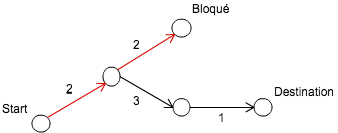
\includegraphics[scale=0.7]{ex.png}
\end{center}

\section*{Question 5 - Arnaud Dethise}

	L'objectif de cette question est d'écrire un algorithme permettant de trouver le meilleur chemin dans un graphe. 
	Il est donc logique d'utiliser l'algorithme de Dijkstra, modifié pour tenir compte des méthodes spécifiques à ce problème dans le calcul du meilleur chemin.
	
	Les deux différences suivantes sont à prendre en compte :
	\begin{itemize}
	\item Le meilleur chemin est celui ayant \textit{la plus grande} bande passante.
	\item Le coût d'un chemin est égal au \textit{coût de l'arête la plus faible} sur ce chemin.
	\end{itemize}
	
	\begin{lstlisting}
	MaxBandWidth(G, a, b) :
		Initialize D[a] = %*$\infty$*) and D[v] = 0 for each vertex v %*$\neq$*) a
		Let a priority queue Q contain all the vertices of G using the D labels as keys
		while b is in Q do
			u = Q.removeMax()
			for each edge (u,v) such that v is in Q do
				if min(D[u], bw(u,v)) > D[v] then
					D[v] = min(D[u], bw(u,v))
					Change the key of vertex v in Q to D[v]
		return D[b]
	\end{lstlisting}

\section*{Question 6 - Arnaud Dethise}

	Remarque : la complexité justifiée ci-dessous est la même que celle de l'algorithme de Dijkstra.

	Soit G contenant $n$ nœuds et $m$ arêtes.
	
	\vspace{0.3cm}
	Première solution :
	\begin{itemize}
	\item Initialiser les valeurs de la liste D : $\mathcal{O}(n)$
	\item Initialiser la priorityQueue Q (heap) : $\mathcal{O}(n~log~n)$
	\item Récupérer $n$ fois l'élément maximal de Q : $\mathcal{O}(n)$
	\item Trouvez tous les vecteurs reliant u à un nœud encore dans Q (matrice d'adjacence) : $\mathcal{O}(m)$
	\item Mettre à jour $m$ fois les clés des vecteurs de Q : $\mathcal{O}(m~log~n)$
	\end{itemize}
	Total : $\mathcal{O}((n+m)~log~n)$, avec $m \leq n^2$.
	
	\vspace{0.3cm}	
	Deuxième solution :
	\begin{itemize}
	\item Initialiser les valeurs de la liste D : $\mathcal{O}(n)$
	\item Initialiser la priorityQueue Q (unsorted list, location aware) : $\mathcal{O}(n)$
	\item Récupérer $n$ fois l'élément maximal de Q : $\mathcal{O}(n^2)$
	\item Trouvez tous les vecteurs reliant u à un nœud encore dans Q (matrice d'adjacence) : $\mathcal{O}(m)$
	\item Mettre à jour $m$ fois les clés des vecteurs de Q : $\mathcal{O}(m)$
	\end{itemize}
	Total : $\mathcal{O}(n^2 + m)$, avec $m \leq n^2$, soit $\mathcal{O}(n^2)$.
	
	\vspace{0.5cm}
	Remarque : Le DSAJ-6 indique qu'une implémentation utilisant la structure \textit{Fibonacci heap} permettrait d'obtenir une complexité asymptotique en $\mathcal{O}(m + n~log~n)$, mais une rapide recherche sur le web indique que cette structure, bien que asymptotiquement plus efficace, est en pratique plus lourde par clé à cause de ses facteurs constants.

% add sections if more questions

\end{document}
